%!TEX root = ../main.tex
\section{Bruce-SLAM adapted to Aracati2017}
\label{sec:chap1}

This chapter describes the \emph{base} method: the Bruce-SLAM system~[1] made
operational, GT-free, on Aracati2017. The original architecture is kept unchanged;
the following sections describe what had to be \textbf{added} for it to work —
on-board odometry and USBL anchoring — then the results under the protocol of
§~\ref{sec:protocole}.

\subsection{Bruce-SLAM pipeline recap}

The front-end extracts ``structure'' points from each sonar image with a
\textbf{SOCA-CFAR} detector; successive scans are aggregated into \textbf{keyframes}
(created beyond a displacement threshold) and registered by sequential \textbf{ICP}
initialised with the odometry. The back-end is a factor graph optimised with
\textbf{iSAM2}~[9]. ``Non-sequential'' loop closures (NSSM) are detected
geometrically: preselection by covariance and estimated overlap, global ICP
initialisation with the \textbf{shgo} optimiser, validation by pairwise consistency
(\textbf{PCM}~[6]). An SSM module (short-term multi-frame registration) refines the
odometry.

\subsection{GT-free odometry: integrating \texttt{/cmd\_vel}}
\label{sec:odom}

Aracati2017 provides no usable inertial odometry; we integrate the on-board velocity
commands (planar unicycle model):
\begin{equation}
\theta_{k+1} = \theta_k + \omega_{z,k}\,\Delta t_k, \qquad
\mathbf{p}_{k+1} = \mathbf{p}_k + v_{x,k}\,\Delta t_k\,[\cos\theta_k,\ \sin\theta_k]^\top
\end{equation}
with the initial state $(\mathbf{p}_0, \theta_0)$ estimated from the
course-over-ground of the first USBL fixes (no ground truth). Since $\omega_z$ is
derived from the compass~[8], the integrated \textbf{heading} is accurate (relative
rotation error $\approx 0$~°/m) but the \textbf{translation} drifts strongly
(commands $\neq$ actual velocities; currents): \textbf{18.3--18.5 m} of anchored ATE
over the mission (orange curve in figures~\ref{fig:bruce-err} and
\ref{fig:bsu-err}). The whole point of the back-end is to correct this translation
without touching the heading.

\subsection{USBL anchoring in the factor graph}
\label{sec:usbl}

The USBL provides noisy absolute position fixes $\mathbf{u}_i$ (multipath, outlier
pings $\sim$73 m off near the transponder). In the code, the USBL can act at three
places, and one must be precise about what is actually enabled:
\begin{itemize}
\item \textbf{frame initialisation} (front-end, once): position of the first fix +
  heading from the course-over-ground of the first fixes — this is the seed
  $(\mathbf{p}_0, \theta_0)$ of §~\ref{sec:odom};
\item \textbf{continuous dead-reckoning correction} (front-end, causal filter):
  \emph{disabled everywhere} in this document;
\item \textbf{position factors in the graph} (back-end): the retained mechanism,
  described below.
\end{itemize}
Enabling both the front-end correction and the back-end factors is a contradictory
double anchoring: the already-corrected odometry fights the factors, with a measured
$\times 3$ ATE degradation. All configurations in this document therefore use
\textbf{seed + back-end only}.

Each fix is associated with the closest keyframe in time ($|t_i - t_k| \le 1$ s,
3 m/s speed gating) and added as a \textbf{robust unary factor on position only}
(the heading is left to the odometry and the loops):
\begin{equation}
\phi_i(\mathbf{X}) = \rho_c\!\left(\frac{\lVert \Pi\,\mathbf{X}_{k(i)} - \mathbf{u}_i \rVert}{\sigma_{\text{usbl}}}\right),
\qquad \rho_c(r) = \tfrac{c^2}{2}\,\log\!\left(1 + \tfrac{r^2}{c^2}\right)
\end{equation}
where $\Pi$ projects the pose onto $(x, y)$ and $\rho_c$ is the Cauchy kernel
(outliers saturate instead of pulling the solution).

\subsection{Results — Bruce-SLAM alone (origin protocol, §~\ref{sec:protocole})}
\label{sec:chap1-res}

Two runs per configuration (repeatability), identical sensor chain everywhere
(odometry of §~\ref{sec:odom}, same configuration files); ``no USBL'' = neither seed
nor factors (fixed-heading start), ``+ USBL'' = seed + back-end factors
$\sigma = 2.5$. Table~\ref{tab:chap1} gathers both configurations; this section reads
Bruce-SLAM alone, §~\ref{sec:chap1-usbl} what the USBL anchor changes.

\begin{table}[H]
\centering
\caption{Chapter 1 — origin-anchored ATE (m), global and per re-anchored section,
and relative errors. Two runs per configuration.}
\label{tab:chap1}
\begin{tabular}{llccccc}
\hline
Config & run & Global ATE & S1 & S2 & S3 & Trans. (\%) \\
\hline
Pure odometry & — & 18.30--18.54 & 5.05 & 11.69 & 7.62 & 32.5 \\
\hline
\multirow{2}{*}{Bruce (SSM+NSSM, no USBL)} & 1 & \textbf{2.33} & \textbf{2.72} & 7.94 & 3.01 & 8.18 \\
                                            & 2 & 3.04 & 2.65 & 6.66 & 2.26 & \textbf{4.83} \\
\hline
\multirow{2}{*}{Bruce + USBL $\sigma{=}2.5$} & 1 & 3.87 & 5.20 & \textbf{4.98} & 2.55 & 23.63$^{1}$ \\
                                              & 2 & 5.76 & 5.60 & 5.74 & \textbf{2.05} & 11.96$^{1}$ \\
\hline
\end{tabular}
\end{table}

With its native loops only (SSM/NSSM), Bruce-SLAM already corrects the odometry by an
order of magnitude:
\begin{itemize}
\item from 18.3 m of raw drift down to \textbf{2.33--3.04 m} of anchored ATE, without
  degrading the heading (median 2.2--3.0°) — figures~\ref{fig:bruce-traj} and
  \ref{fig:bruce-err};
\item per re-anchored section: 2.65 / 6.66 / 2.26 m (run 2,
  figure~\ref{fig:bruce-sections}) — S2 concentrates the drift, with few revisits to
  correct it;
\item the map is correct, not just sharp: point cloud at \textbf{0.09 m} (median)
  from the cloud re-rendered at the ground-truth poses, p90 0.70 m
  (figures~\ref{fig:bruce-map} and \ref{fig:bruce-cloudgt}).
\end{itemize}

\begin{figure}[H]
\centering
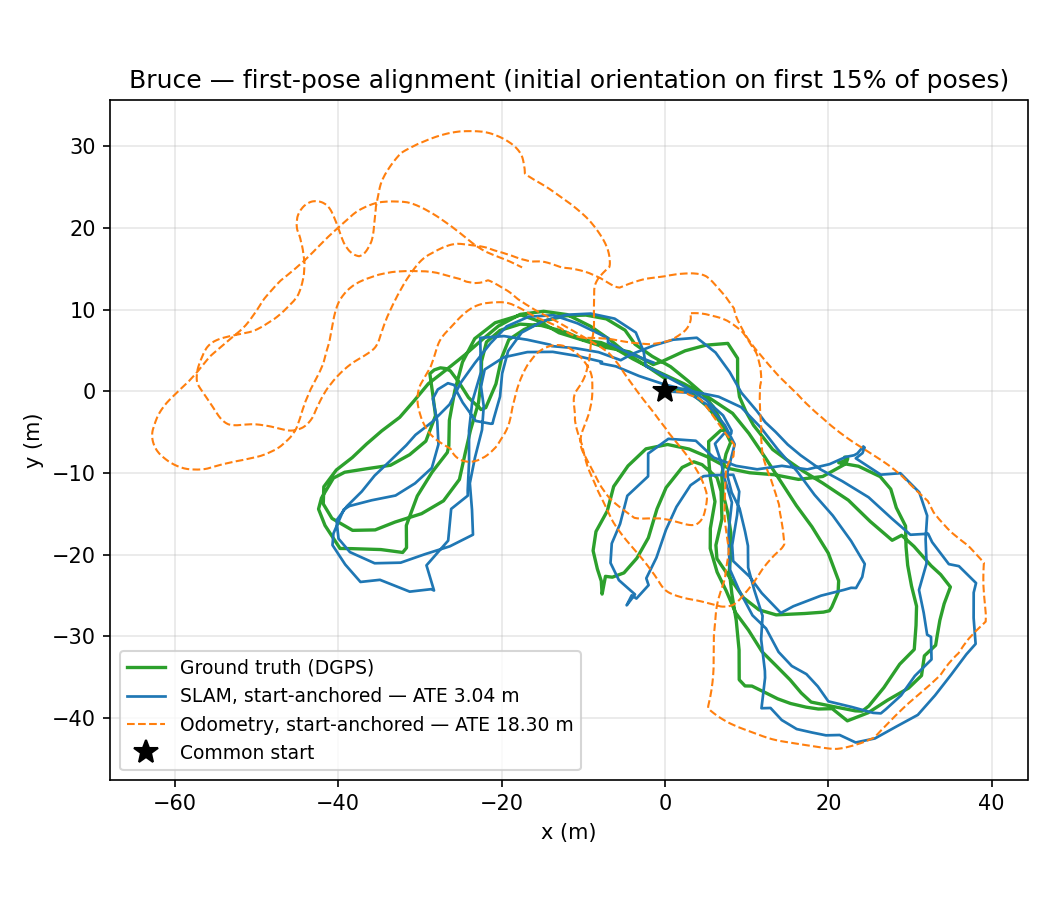
\includegraphics[width=0.72\textwidth]{Image/Bruce_traj_origine.png}
\caption{Bruce-SLAM alone (run 2) — trajectories anchored at the common start
(star): DGPS ground truth, SLAM, pure odometry.}
\label{fig:bruce-traj}
\end{figure}

\begin{figure}[H]
\centering
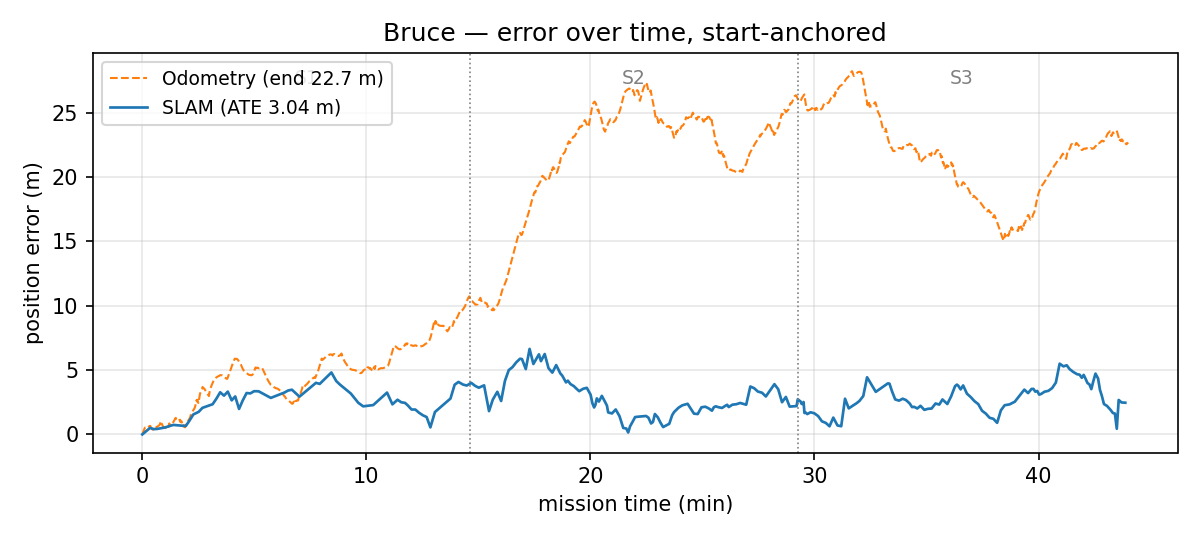
\includegraphics[width=0.9\textwidth]{Image/Bruce_err_time_origine.png}
\caption{Bruce-SLAM alone — position error over the mission, origin-anchored
convention. The odometry (orange) accumulates $\sim$20 m; SLAM stays bounded. Grey
dotted lines: section boundaries.}
\label{fig:bruce-err}
\end{figure}

\begin{figure}[H]
\centering
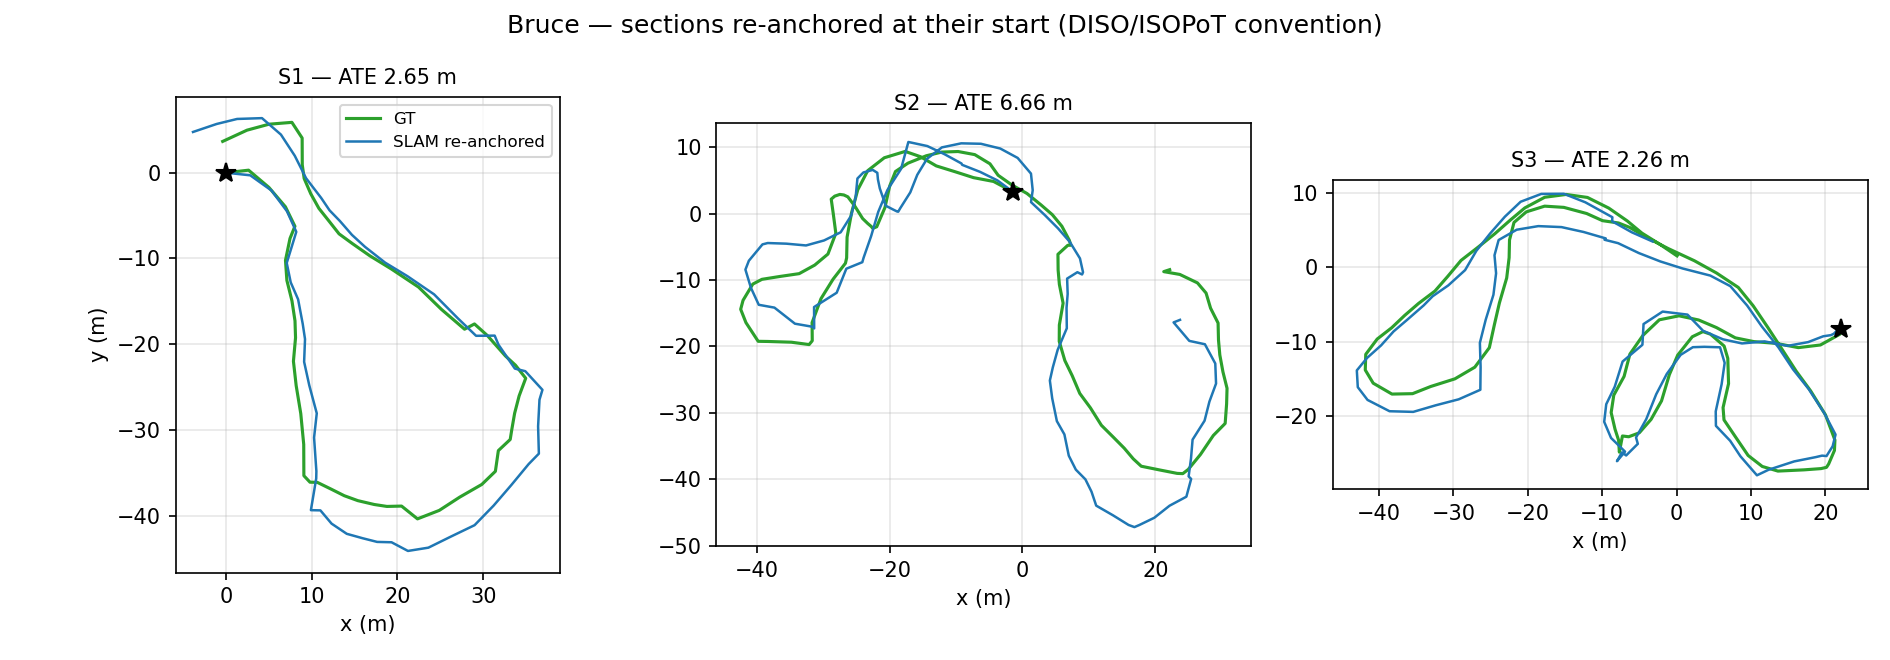
\includegraphics[width=\textwidth]{Image/Bruce_sections_origine.png}
\caption{Bruce-SLAM alone — each section re-anchored at its own start (DISO/ISOPoT
convention). Per-section ATEs do not average to the global one: each section
inherits an independent local anchor (§~\ref{sec:protocole}b).}
\label{fig:bruce-sections}
\end{figure}

\begin{figure}[H]
\centering
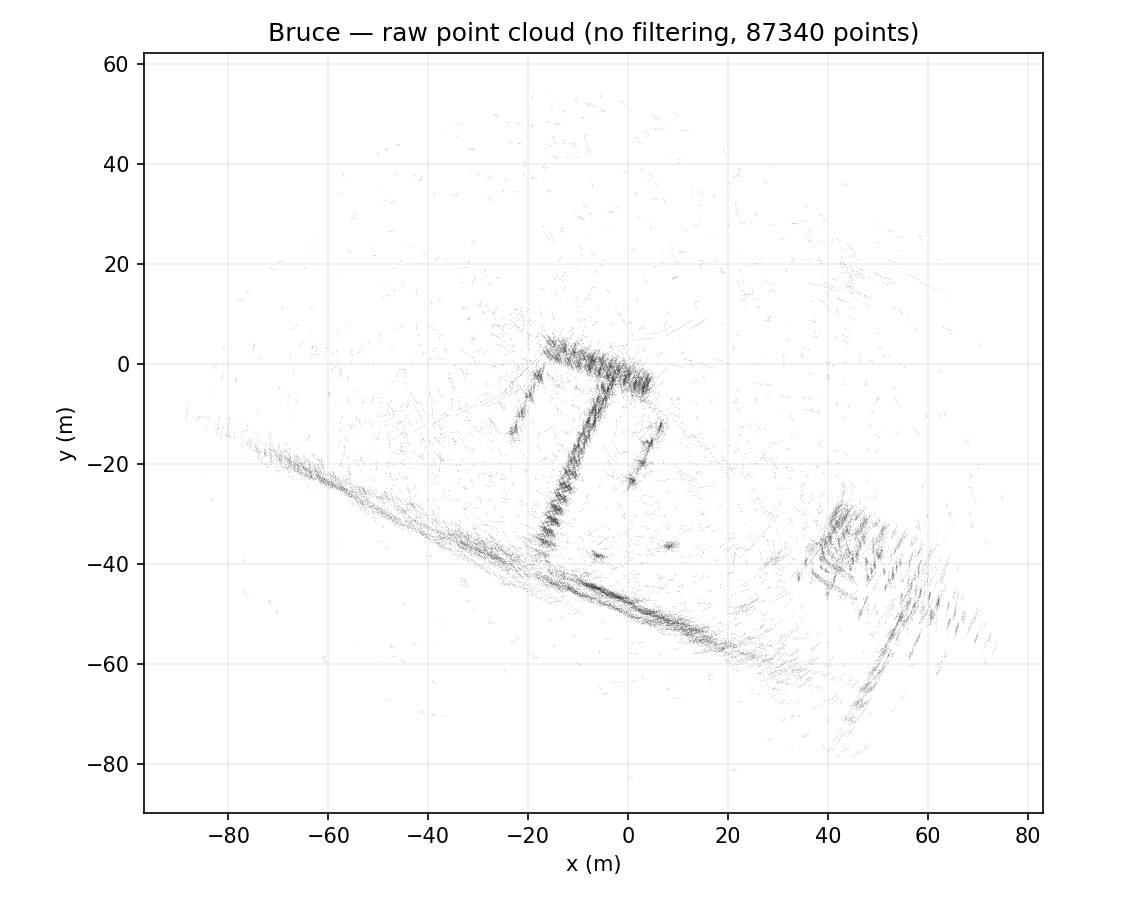
\includegraphics[width=0.8\textwidth]{Image/Bruce_pointcloud_map.png}
\caption{Bruce-SLAM alone — raw map (full point cloud, no filtering): the T-shaped
dock and the marina pontoons.}
\label{fig:bruce-map}
\end{figure}

\begin{figure}[H]
\centering
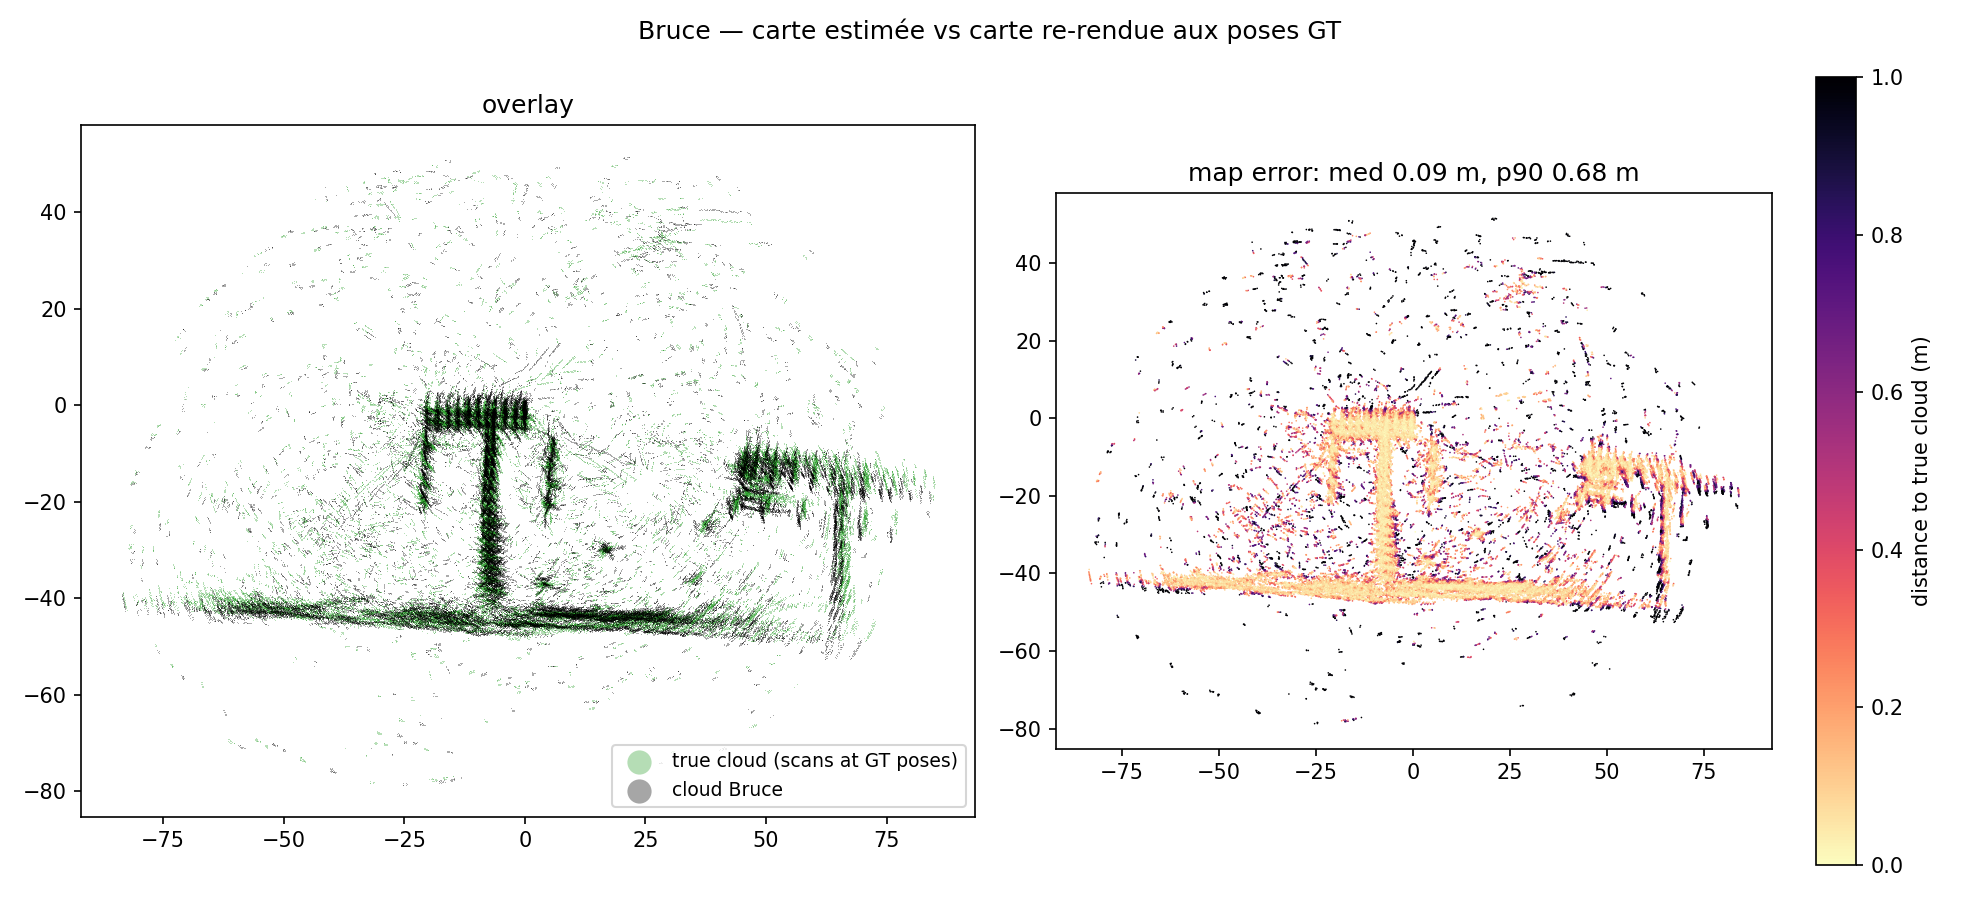
\includegraphics[width=\textwidth]{Image/Bruce_cloud_vs_gt.png}
\caption{Bruce-SLAM alone — estimated map against the ``true'' map (same detections
re-rendered at the ground-truth poses: DGPS position, compass heading —
§~\ref{sec:protocole}e). Median 0.09 m, p90 0.70 m.}
\label{fig:bruce-cloudgt}
\end{figure}

\subsection{Adding the USBL anchor}
\label{sec:chap1-usbl}

The same system with the USBL anchor of §~\ref{sec:usbl} (seed + back-end factors,
$\sigma = 2.5$) gives figures~\ref{fig:bruce-usbl-traj} to
\ref{fig:bruce-usbl-sections}. Two effects, in opposite directions:

\begin{itemize}
\item \textbf{$^{1}$The seed artefact on the anchored metric.} The USBL runs show a
  \emph{higher} Trans.~\% and global anchored ATE (3.87--5.76 m) than Bruce alone —
  a measured artefact, not a flaw of the anchor: the initial heading is estimated
  from the course-over-ground of the first USBL fixes (noisy), and in this method
  nothing corrects it afterwards (the USBL factors only touch $x,y$). The convention
  offset $\beta$ drawn at start varies from run to run ($\beta$ = 90.3° $\to$ Trans
  4.83~\%; 100.5° $\to$ 11.96~\%; 112.4° $\to$ 23.63~\% — direct correlation), and
  the RE, which expresses displacements in the frame of \emph{each} pose, takes
  $\sim$1~\%/degree of offset. Bruce alone starts from a fixed heading (no estimated
  seed), hence a nominal $\beta$.
\item \textbf{Per section, the anchor pays off after S1.} With each section properly
  re-anchored, Bruce + USBL wins S2 (4.98--5.74 m against 6.66--7.94) and S3
  (\textbf{2.05--2.55 m} against 2.26--3.01), where the drift of Bruce alone is no
  longer corrected by revisits; S1 and the global figure pay the noisy heading seed.
  The map metric is unchanged (0.09 m median): the anchor moves the trajectory, not
  the local consistency of the scans.
\end{itemize}

\begin{figure}[H]
\centering
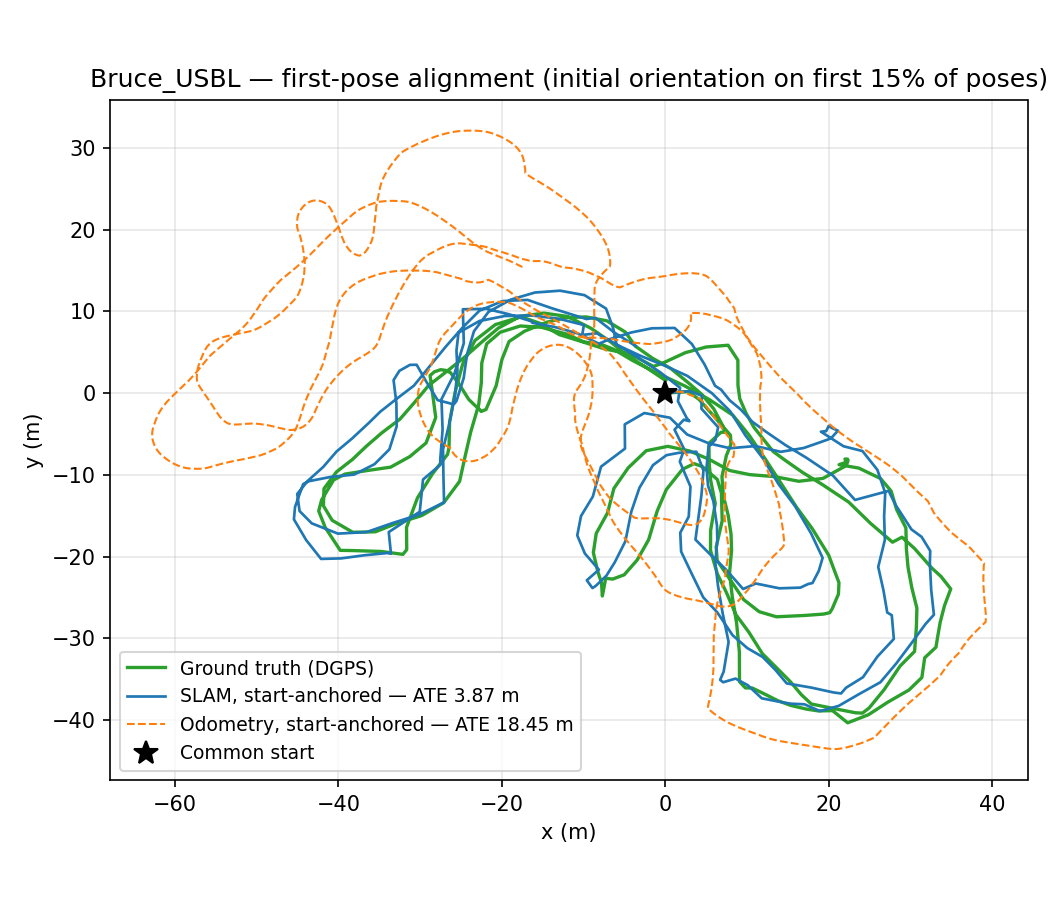
\includegraphics[width=0.72\textwidth]{Image/Bruce_USBL_traj_origine.png}
\caption{Bruce + USBL $\sigma{=}2.5$ (run 1) — trajectories anchored at the common
start. The global anchored ATE (3.87 m) is dominated by the noisy USBL heading seed
(§~\ref{sec:chap1-usbl}).}
\label{fig:bruce-usbl-traj}
\end{figure}

\begin{figure}[H]
\centering
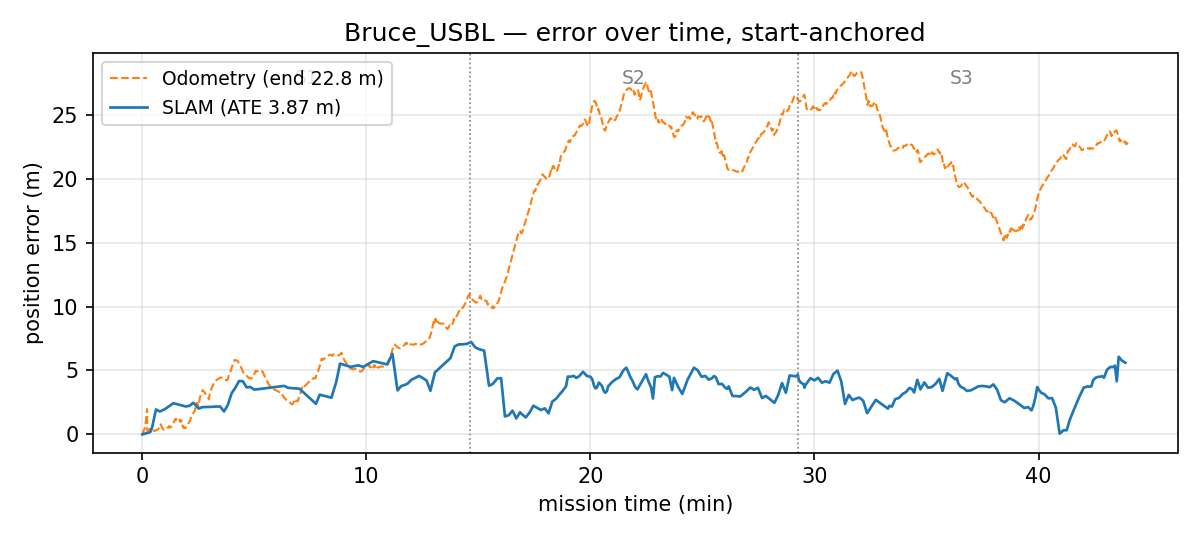
\includegraphics[width=0.9\textwidth]{Image/Bruce_USBL_err_time_origine.png}
\caption{Bruce + USBL — position error over the mission (origin-anchored). The
initial heading offset spreads over the whole mission; per-section re-anchoring
(figure~\ref{fig:bruce-usbl-sections}) removes it.}
\label{fig:bruce-usbl-err}
\end{figure}

\begin{figure}[H]
\centering
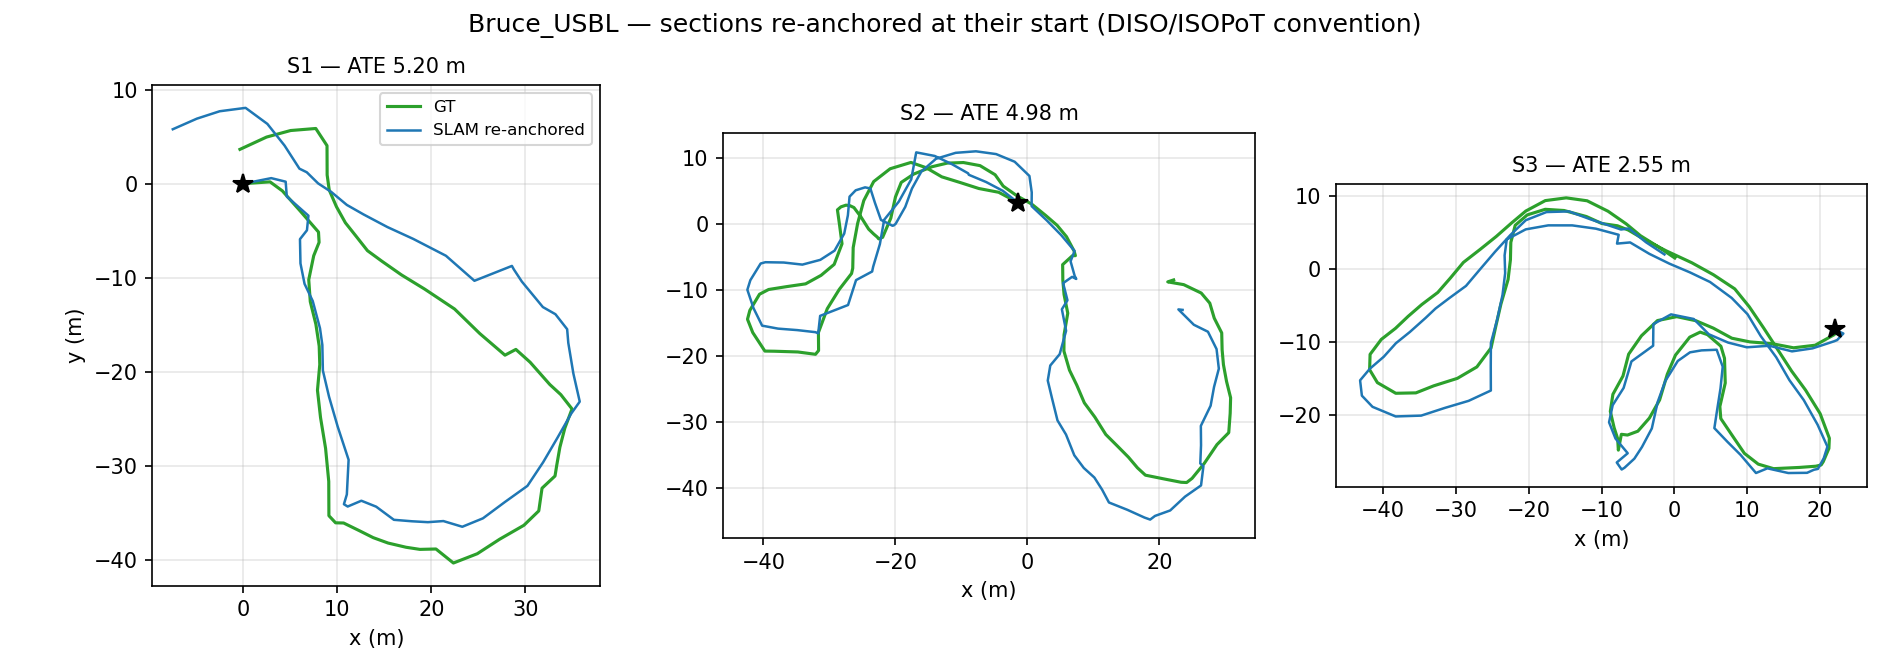
\includegraphics[width=\textwidth]{Image/Bruce_USBL_sections_origine.png}
\caption{Bruce + USBL — sections re-anchored at their start: S3 = 2.55 m and S2
improve over Bruce alone, where the anchor compensates the scarcity of loops.}
\label{fig:bruce-usbl-sections}
\end{figure}
